\documentclass{article}
\usepackage[utf8]{inputenc}
\usepackage{lipsum}                     % Dummytext
\usepackage{hyperref}
\usepackage{xargs}                      % Use more than one optional parameter in a new commands
\usepackage[pdftex,dvipsnames]{xcolor}  % Coloured text etc.
\usepackage{graphicx}
\usepackage{verbatim}
\usepackage{float}

\hypersetup{
    colorlinks=true,
    linkcolor=blue,
    filecolor=magenta,      
    urlcolor=cyan,
}

\usepackage[english]{babel}
\emergencystretch=1pt
\usepackage[justification=centering]{caption}
\graphicspath{{Pictures/} }

\usepackage[colorinlistoftodos,prependcaption,textsize=tiny]{todonotes}
\newcommandx{\unsure}[2][1=]{\todo[linecolor=red,backgroundcolor=red!25,bordercolor=red,#1]{#2}}
\newcommandx{\change}[2][1=]{\todo[linecolor=blue,backgroundcolor=blue!25,bordercolor=blue,#1]{#2}}
\newcommandx{\info}[2][1=]{\todo[linecolor=OliveGreen,backgroundcolor=OliveGreen!25,bordercolor=OliveGreen,#1]{#2}}
\newcommandx{\improvement}[2][1=]{\todo[linecolor=Plum,backgroundcolor=Plum!25,bordercolor=Plum,#1]{#2}}
\newcommandx{\thiswillnotshow}[2][1=]{\todo[disable,#1]{#2}}

\usepackage{setspace}
\doublespacing

\title{Sensor Node Documentation}
\author{Isaak Cherdak}
\date{March 2017}

\begin{document}

\maketitle

\tableofcontents

\section{Sensor Node}

\subsection{The Information Infrastructure}

Sensor Node will function as a component of the Information Infrastructure of a separate micro grid project. The purpose of a Information Infrastructure is to facilitate the efficient and secure flow of data. It is responsible for communicating with sensors, actuating devices, etc and providing this data securely and in real time to grid workers.

\subsection{What is Sensor Node and why is it useful?}

The current version of Sensor Node is a library written by Isaak Cherdak but originated from Sargis Yonan's original version. The library's purpose was originally to be used in a distributed system of sensors communicating with a database but it actually has many more applications. In this case we are using it as a single node since we will only need one device to run all of the sensors and have plans to design a data visualization system or integrate with an existing one so as to be able to conveniently get information in real time. In addition, Sensor Node is designed for two way communication since version 2 for things such as actuators (which has thus far been implemented using LEDs) so the user interface providing data visualization will ideally provide this functionality as well. Note that all versions of Sensor Node were written for the Arduino AtMega 2560.

This paper will be discussing the third version of Sensor Node. The first version of Sensor Node was created by Sargis Yonan and simply allowed continuous data output for one kind of sensor at a hard-coded frequency (usually 1 Hz). The first version is currently in a branch called "legacy" but will eventually be moved to "v1". The second version was created by Isaak Cherdak and allowed for communication with multiple devices but their locations were predefined and although it was designed with performance in mind, it wasn't designed very well to allow for easy integration with new kinds of devices. The second version is in a branch called "legacy\_v2" and will eventually be moved to "v2". Version 3 was also written by Isaak Cherdak and improved on the issues of version 2. In version 3 it is possible to easily add code to interface with new devices, add and remove devices \textit{during run-time} on any pin you would like and easily see which devices are currently installed and registered with the board running Sensor Node. This is accomplished by standardizing the kinds of values that each device, or as the library calls it, \textbf{module} must support. One of the biggest core design choices was to categorize every device as having four kinds of commands: \textbf{init}, \textbf{read}, \textbf{write}, and \textbf{destroy}. Currently the master branch points to the third version. Sensor Node version 3 has just reached it's first minimum-spec complete state which has been appropriately labeled v3.0.0 alpha. Finally, note that when discussing something about the library, unless otherwise specified assume that it is in regards to Sensor Node v3.0.0.

\subsection{Currently Implemented Modules}
\label{subsec:sensor_node_current_modules}

Some Modules already have been implemented and integrated into Sensor Node, further demonstrating the effectiveness of the library's simple design. Note that the wiring of these devices will be illustrated in \autoref{subsec:sensor_node_wiring}.

\subsubsection{Actuator}

The Actuator module was created by copying the format of the default module library and simply replacing the code as appropriate within the four standard functions. A quick comparison of module.c and actuator.c can demonstrate how simple this was to do. In addition, the actuator module is a very simple concept: a device that can be turned on or off. In our case we used LEDs as the physical devices that operated as actuators. This will be useful if we want to have a panel of LEDs to display the status of various systems inside a facility. Finally, this is also an example of a library that particularly requires two way communications between the data visualisation system. For more information on this, please refer to \autoref{subsubsec:sensor_node_data_visualisation}

\subsubsection{Temp\_Sensor}

The Temp\_Sensor module was created by taking its code from Sensor Node v2.0.0 and adding support for the init and write functions. It should be noted that this library is \textit{atrocious} and will likely be rewritten in the near future. It features terrible things like half-second delays and an unnecessary length of code for the provided functionality that more than doubled the size of the binary through inclusion into Sensor Node v3.0.0. The origins and original author of the code are currently unknown but we know that it was present during Sensor Node v1. We are using the DS18B20 Temperature Sensor currently.

\subsection{Physical Wiring}
\label{subsec:sensor_node_wiring}

Note that this wiring diagram is "loose" in the sense that I don't specify a required location for every device to be wired to. This is obviously because Sensor Node v3.0.0 is modular and allows you to change these locations during runtime. I will however complement the diagram with a set of commands needed to create the devices on the running instance given the locations that you would like them to have. Also note that this is the layout that we used upon completion of v3.0.0 and this may change in later versions depending on the number of additional modules supported. For more information on how to use these commands please take a look at \autoref{subsec:sensor_node_usage}. The illustration of the wiring can be found in \autoref{Sensor Node Wiring}. The commands to configure Sensor Node to use this setup can be found in \autoref{Sensor Node Wiring Commands} (where the locations, \$WLOC to \$ZLOC, must be determined depending on where you place the devices).

\begin{table}[h!]
    \centering
        \begin{tabular}{|c|}
            \hline
            c TEMP\_SENSOR \$WLOC\\
            c ACTUATOR \$XLOC\\
            c ACTUATOR \$YLOC\\
            c ACTUATOR \$ZLOC\\\hline
        \end{tabular}
        \caption{Commands to create the devices in the order they appear from left to right in \autoref{Sensor Node Wiring}}
        \label{Sensor Node Wiring Commands}
\end{table}

\begin{figure}[h!]
    \centering
        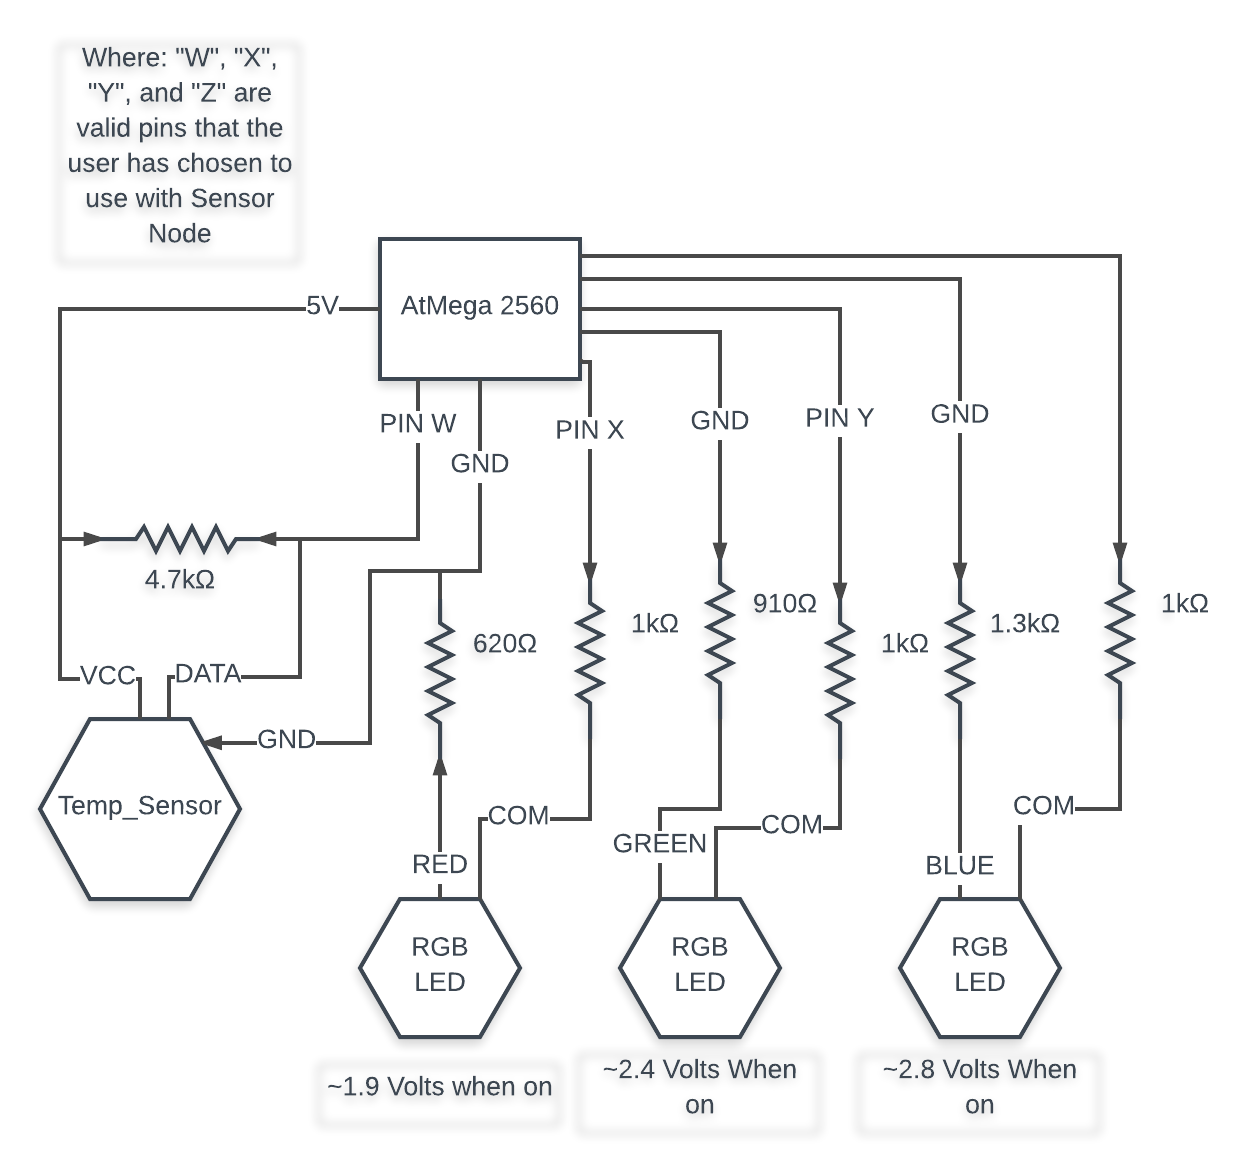
\includegraphics[width=\linewidth]{Sensor_Node_System_Physical_Wiring.png}
        \caption{Sensor Node Wiring}
        \label{Sensor Node Wiring}
\end{figure}

\subsection{Usage}
\label{subsec:sensor_node_usage}

For more details on how the system and commands work, please visit \autoref{subsec:sensor_node_docs}. For more details on the usage of specific modules, please visit \autoref{subsec:sensor_node_current_modules}

%format the following better
\subsubsection{Key}

You can expect to see the terms in \autoref{Usage Section Key Terms} throughout the Usage section.
\\

\begin{table}[h!]
    \centering
  \begin{tabular}{ | l | l | }
    \hline
    [ ] & white-space \\ \hline
    \%PORT & PXN \\ \hline
    \%DEV\_STR & string describing the device type \\ \hline
    \%I & device index \\ \hline
    \%WRITE\_STR & the command to send to write \\
    \hline
    \end{tabular}
    \caption{Key Terms for Usage Section}
    \label{Usage Section Key Terms}
\end{table}

\subsubsection{Create}

This command creates a new device of type \%DEV\_STR at location PXN where 'P' has no meaning, X is the letter of the register (IE: 'A' in "PA0") and N is the bit of the register we would like to use (IE: '0' in "PA0"). After creation, "init" is called on the new device. Note that the index the device is placed on upon creation can later be determined with the "map" command. This command's syntax is most likely to change. Please refer to \autoref{subsubsec:sensor_node_multiple_pins} for more information.
\\
\textit{Syntax: }\textbf{c}[ ]\%DEV\_STR[ ]PXN

\subsubsection{Initialize}

This command can be overwritten by a module. By default it will return a generic string saying that "init" was called on device \%I of type \%DEV\_STR. In short, it will call the "init" command on device \%I and the main function will print the returned string.
\\
\textit{Syntax: }\textbf{i}\%I

\subsubsection{Read}

This command can be overwritten by a module. By default it will return a generic string saying that "read" was called on device \%I of type \%DEV\_STR. In short, it will call the "read" command on device \%I and the main function will print the returned string.
\\
\textit{Syntax: }\textbf{r}\%I

\subsubsection{Write}

This command can be overwritten by a module. By default it will return a generic string saying that "write" was called on device \%I of type \%DEV\_STR with string \%WRITE\_STR. In short, it will call the "write" command on device \%I and the main function will print the returned string.
\\
\textit{Syntax: }\textbf{w}\%I[ ]\%WRITE\_STR

\subsubsection{Destroy}

This command can be overwritten by a module. By default it will return a generic string saying that "destroy" was called on device \%I of type \%DEV\_STR. In short, it will call the "destroy" command on device \%I and the main function will print the returned string.
\\
\textit{Syntax: }\textbf{d}\%I

\subsubsection{Kill}

This command will remove device \%I from the current instance configuration. Before doing so, it also calls destroy on device \%I.
\\
\textit{Syntax: }\textbf{k}\%I

\subsubsection{Map}

This command prints information about the configuration of the current instance. Currently, this information simply shows which types of devices are located on which indices but eventually it will also display the on-board location(s) taken up by the device, the different kinds of available device types, and possibly an additional custom string that each device even within types may provide for additional identification or status purposes.
\\
\textit{Syntax: }\textbf{m}

\subsection{Documentation}
\label{subsec:sensor_node_docs}

\subsubsection{Overview}
\label{subsubsec:sensor_node_overview}

This section will talk about details that the general user may not be interested in but a programmer seeking to utilize our libraries or expand them will need to know. We will be designing with backwards compatibility in mind for at least version 3.0.0. As of Sensor Node v3.0.0 a device operating the firmware allows you to do 7 fundamental operations. Three of these operations are the same no matter which modules are installed: "map" ('m') which displays the current system configuration, "create" ('c') which adds a new device at a specified pin to the running instance, and "kill" ('k') which removes a device from the running instance. Then there are four commands that are standardized and hence differ between different types of devices: "init" ('i') which initializes a device, "read" ('r') which reads data from a device, "write" ('w') which sends a string to a device, and "destroy" ('d') which should set the pin the device was running on to the state that it was in before initializing the device. Note that if overwriting one of these four standardized commands in a module, you must return a valid string because \textbf{the returned parameter will be sent to a uart\_puts command}. Note that this is done largely because it is better to standardize the majority of functionality in one place and have every module be as simple as possible for ease of implementation and integration. If you would like to print a message, please simply create the string you want displayed and it will be appropriately printed. Finally, Sensor Node comes with three libraries that must be included: a UART library, a parser, and the module standard library. I will conclude the documentation by discussing what the core operation of Sensor Node (The contents of main.c) is responsible for.

\subsubsection{UART library}

The UART library is made up of uart.c and uart.h. The library provides an interface with the on-board uart which currently allows communications through a serial terminal. It provides the same functions you would expect when programming in a normal computer environment like printf() and gets(). This library also features two interrupts: one always triggers when data is received while the other is enabled only when there is data to be transmitted and triggers when the data register is empty.

\subsubsection{Parser library}

The parser encapsulates all of the arguments that we would expect from a command. It doesn't print anything directly either since that would be bad practice: instead the core library prints messages related to the return of the parser. The parser will return with the command parameter being set to NULL in the scenario that it detects an error. It doesn't handle all errors. Some error handling like checking for valid index or string types are considered in the core library since the parser doesn't have access to the information necessary to check these things. When the parser successfully returns, it will have a character saved depending on the command that was correctly executed. In the case of 'i'/'r'/'d'/'k' it simply expects a number and will set the device\_index to \%I. In the case of 'w' it sets device\_index to the \%I and ret\_str to the \%WRITE\_STR. In the case of 'c', it sets the ret\_str to \%DEV\_STR, address\_index to (X - 'A'), and reg\_bit to (N - '0'). Finally, In the case of 'm', it simply returns. Unless specifically defined for a specific case, you should assume that the value for a given parameter of a Parser object is undefined. To see the expected syntax for Sensor Node, please visit \autoref{subsec:sensor_node_usage}.

\subsubsection{Module library}

This library standardizes the parameters that are expected for a given module for Sensor Node. When creating a new module, you should override every parameter of the module struct that you can. For example, you definitely will want to override the type\_num because otherwise, when a device of that type is created, it will be the default type which is -1 and hence cause a segmentation fault because that index of the maps in the core library does not exist. For more information check out \autoref{subsubsec:sensor_node_core_library}. It should be noted that some things are likely to be changed such as the way the information for pins is saved (this particular concern is addressed in \autoref{subsubsec:sensor_node_multiple_pins}). The standard set by this library is what allows us to make simplified assumptions about how we can use every library. Also note that printing shouldn't happen in any module. The functions pointed to by a module struct must return a string that will be printed by the core library otherwise, per the current design a segmentation fault will occur.

\subsubsection{Core library}
\label{subsubsec:sensor_node_core_library}

This library is the control system of Sensor Node. It keeps all of the maps such as: type index to creation function, type index to type string, device index to device, etc. It also is in charge of receiving data from the UART and requesting specific information from that data through the parser. Once it receives the data, it acts upon one of the 7 commands. For general information on these commands refer to \autoref{subsubsec:sensor_node_overview} or for usage refer to \autoref{subsec:sensor_node_usage}. The library also is responsible for printing to the UART things like errors received and strings returned from function calls to various modules. A block diagram demonstrating the interconnection of the high level system architecture can be found in \autoref{Sensor Node Architecture}

\begin{figure}[h!]
    \centering
        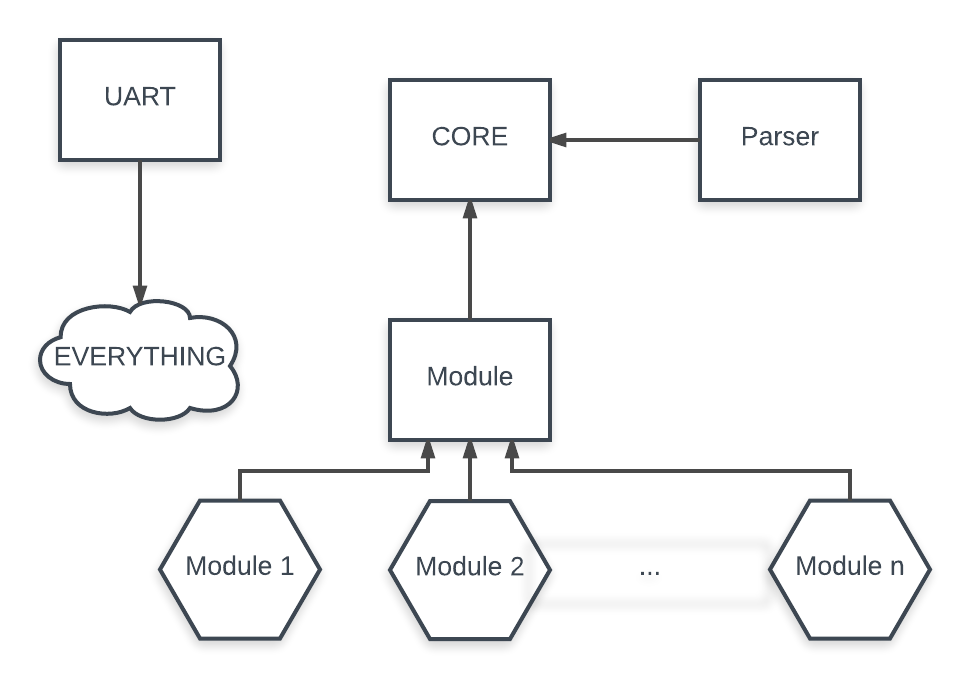
\includegraphics[width=\linewidth]{Sensor_Node_Architecture.png}
        \caption{Sensor Node Architecture}
        \label{Sensor Node Architecture}
\end{figure}

\subsection{Issues}
\label{subsec:sensor_node_issues}

\subsubsection{Devices Requiring Multiple Pins}
\label{subsubsec:sensor_node_multiple_pins}

Sensor Node currently doesn't consider the additional information that may need to be saved when dealing with multiple devices on the same pins (since interfaces like I2C should be supported to work with multiple devices) but with the current progress of the library it shouldn't be a problem to add this functionality.

\subsubsection{Interrupt Interferences}

This is more of a potential issue that hasn't been considered and has yet to cause any problems. The point is that there may be modules or general additions to Sensor Node that utilize additional interrupts. This shouldn't necessarily be encouraged but it certainly \textit{shouldn't be discouraged}. Although the design has been considerate for an embedded environment, it hasn't been considering possible problems that may arise with larger numbers of interrupts. Basically, the key thing to be considerate of is atomic operation (not yet actualised) and limiting the amount done during an interrupt service routine (actualised).

\subsection{Future Work}
\label{subsec:sensor_node_future_work}

Sensor Node is always being improved upon but we have very concrete plans for our next steps that we expect to complete by the end of spring 2017. The plans will be extended even more at that time for the final version of this report.

\subsubsection{Data Visualisation System}
\label{subsubsec:sensor_node_data_visualisation}

We plan to either create our own or integrate with an existing data visualisation system. We have two major concerns: that the system be dynamic and scalable so as to match the devices running for any given instance as well as to be full duplex or to allow reading data from as well as writing data to Sensor Node. Because this is a tall order, few existing systems provide this functionality so we are leaning on creating our own. We are considering two existing systems for possible integration however: SEADS backend and a data visualisation system made for a farm sensor module by Babandeep Singh and a Computer Science senior design team. Currently, this is by far the largest concern in terms of expected time and scale for implementation. we have for the Information Infrastructure of our grid.

\subsubsection{Mobile Data Module}

We are going to need Sensor Node to communicate over the web to receive commands and send data to a backend server. We have decided to move away from hot spot and wifi connections for a number of reasons. The major reasons were that we would have to worry less about bandwidth limitation if the data is exclusively used by the device, we wouldn't have to worry about powering an entire hot spot, and we can pay less since the data rates needed solely for communications with a backend server will be meager. Thus we will be looking into the use of Arduino shields that can communicate with the board directly. We considered the Adafruit FONA 3g initially but seeing as it currently doesn't have the libraries for TCP/IP and HTML, we will have to go with the Adafruit FONA 800. In the future, once the libraries for the FONA 3g are completed it would be best if someone added code to utilize it instead. The major concern is that the FONA 800 is only uses 2g but at least it costs 40 dollars as opposed to the FONA 3g's price tag of 80 dollars. Example code is provided for the FONA 800 to do anything from making calls, texting, and connecting to the web.

\subsubsection{Humidity Sensor Module}

The code for the module already exists but it hasn't been integrated into Sensor Node yet. This should be quick and simple as I have demonstrated with the ease of integration for modules like the temperature sensor. For more information, refer to \autoref{subsec:sensor_node_current_modules}. We are using the DHT11 as hardware.

\subsubsection{Light Sensor Module}

The module previously used for sensing light utilized the I2C interface. The reason it will likely not be used however is a consequence of bureaucracy. Since the only one we could find was not on an approved website, we decided it will be a hassle to attempt to purchase it through our project's funding and have decided to look for a different one instead.

\subsubsection{CAN transceiver module}

The module will likely be created after the multiple pin fix described in \autoref{subsubsec:sensor_node_multiple_pins}. The module will be based off the MCP2551-E/P CAN transceiver which uses TTL (we initially purchased it thinking it was for SPI but we got it working with TTL so it's not an issue).

\subsubsection{RS232 module}

The module will work with RS232 primarily for communicating with the morning star systems already in the grid. This is a stretch goal as this data isn't particularly necessary.

\subsubsection{Self Documenting Code}

Through the use of Doxygen, as long as the code adheres to their standards for automatic documentation generation, we will easily be able to generate a documentation for the code. Of course, this will not suffice alone and hence the high-level documentation is presented in this report.

\subsubsection{Ideal Deliverable of Modules}

In the ideal case, all of our future work would be completed by the end of Spring 2017. This is illustrated in \autoref{Sensor Node Deliverable}

\begin{figure}[h!]
    \centering
        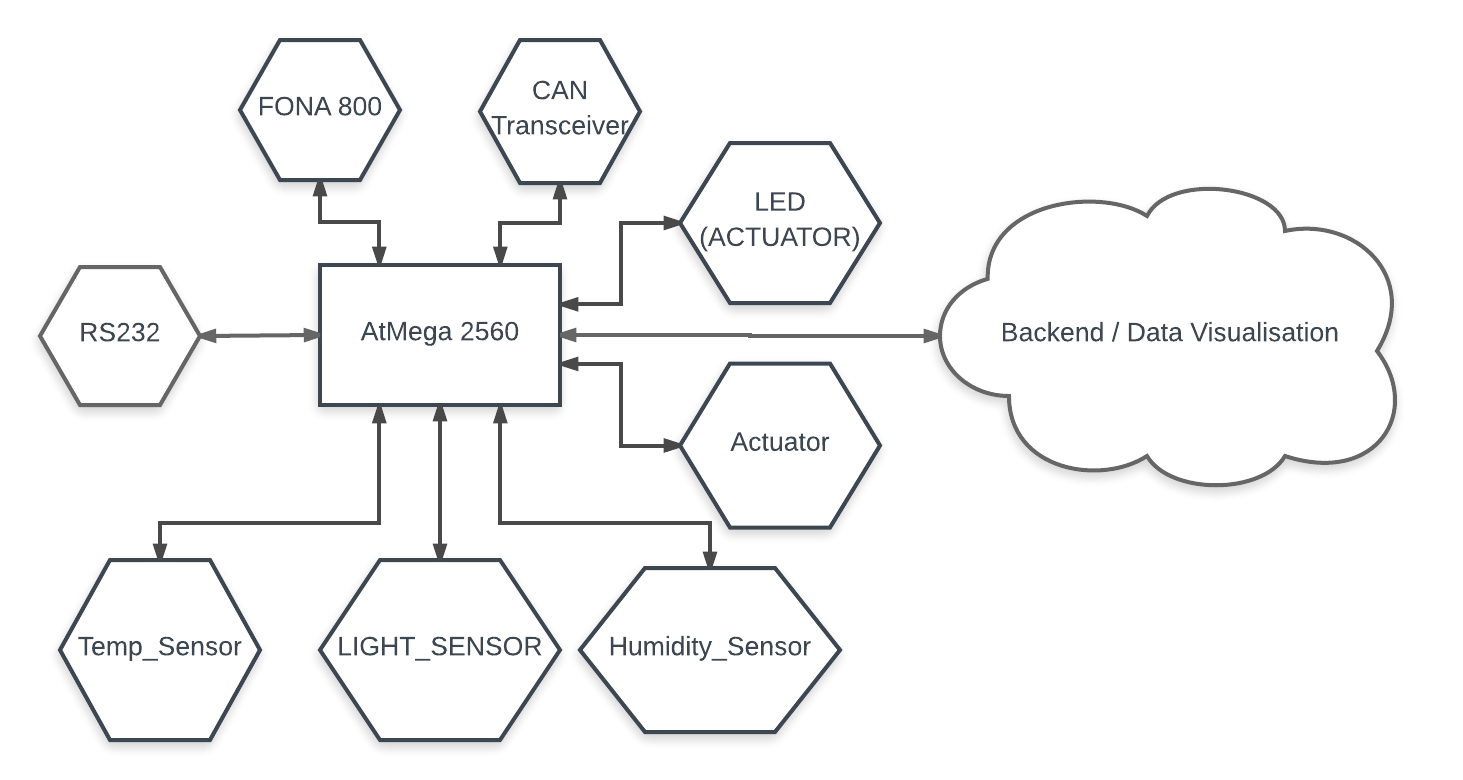
\includegraphics[width=\linewidth]{Sensor_Node_Deliverable.png}
        \caption{Sensor Node Deliverable}
        \label{Sensor Node Deliverable}
\end{figure}

\subsection{Useful Links}

The Sensor Node library can be found here:
\href{https://github.com/legendddhgf/SensorNode}{SensorNode Library}\\

\end{document}
